\section{Browserimplementierungen}

Der Browser Namespace implementiert die einzelnen Browser die in der Sidebar angezeigt werden.
Alle Klassen in diesem Namespace gehören nach dem MVC Paradigma der Controllerebene an - sie sind gewißermaßen der Kleber zwischen der Präsentation und der Logik.
Wie die meisten anderen peripheren Klassen erben diese von \emph{AbstractClientUser} um Änderungen von diesem empfangen zu können. Dies wird im Folgenden nicht mehr explizit erwähnt.

\subsection{Hauptklassen}
\subsubsection{BasePopup}
%Klassendiagramm zu Nutzern von BasePopup

Alle Klassen die ein ,,Kontextmenü'' anzeigen wollen leiten von dieser Klasse ab.
Die ableitende Klasse muss den Konstruktor von BasePopup das Widget übergeben welches das Kontextmenü anzeigen soll, 
und sie erwartet eine von UI Definition des Menüs, dessen Struktur von Gtk+ vorgegeben wird.
Eine beispielhafte UI Definition sieht folgendermaßen aus:
\begin{verbatim}
   <ui>
     <popup name='QueuePopupMenu'>
       <menuitem action='q_remove'/>
       <menuitem action='q_clear'/>
       <separator />
       <menuitem action='q_add_as_pl'/>
     </popup>
   </ui>
\end{verbatim}

Die ableitende Klassen definieren dann das Aussehen des Menüs über die vererbte Funktion menu\_add\_item():
\begin{verbatim}
   // Durch BasePopup definiert
   void menu_add_item(Glib::RefPtr<Gtk::Action>& action,
                      Glib::ustring item_name,
                      Glib::ustring item_label,
                      Glib::ustring item_tooltip,
                      Gtk::StockID icon);
                      
  // Angewendet in einer abgeleiteten Klasse:
  menu_add_item(m_ActionClear,"q_clear","Clear","Clear Queue",Gtk::Stock::CLEAR);
\end{verbatim} 

Zudem bietet die Klasse eine get\_action() Methode um die eigentliche Implementierung der Aktionen nicht in die abgeleitete Klasse machen zu müssen. 

Im Code könnte das so aussehen:
\begin{verbatim}
    /* mp_Popup ist die Instanz einer von BasePopup abgeleiteten Klasse */
    mp_Popup->get_action("q_clear").connect(<funktionspointer>);

    ...

    void Queue::clear_queue_action(void)
    {
        ...
    }
\end{verbatim}


\subsubsection{Database}
\paragraph{Database}
Diese Klasse kontrolliert die Anzeige des Datenbankbrowsers. Sie leitet sich daher von \emph{AbstractBrowser} ab um sich bei der Browserliste registrieren zu können.
Um die Methoden des \emph{AbstractItemGenerator} Interface zu benutzen leitet es zudem von \emph{AbstractItemlist} ab und implementiert daher eine add\_item() Methode. 
Diese fügt letzlich die gewonnenen Items seinem Model (einem Gtk::ListStore) hinzu.

\paragraph{DatabasePopup}
Eine Klasse die von BasePopup ableitet und das Popup definiert, das auftaucht wenn man im Databasebrowser ,,rechtsklickt''.
Sie bietet die folgenden Aktionen an, die man über die Methode get\_action() abgefragt werden kann.
Dadurch kann auf folgende Aktionen reagieren kann:
\begin{itemize}
\item ,,db\_add'' (Fügt Auswahl zum Ende der Queue hinzu)
\item ,,db\_add\_all'' (Fügt alles zum Ende der Queue hinzu)
\item ,,db\_replace'' (Dasselbe wie db\_add, leert aber Queue vorher)
\item ,,db\_update'' (Sendet Server einen Updatehinweis)
\item ,,db\_rescan'' (Sendet Server einen Rescanhinweis)
\end{itemize}

\paragraph{DatabaseCache}
Ein Zwischenspeicher für die im Databasebrowser angezeigten Ordner und Dateien. 
Sie setzt das Proxy-Pattern für MPD::Client um und erbt daher von der \emph{AbstractItemGenerator} um sich als Client ausgeben zu können.
Sie implementiert daher die fill\_filelist() Methode vor, lässt aber die anderen Methoden ohne Implementierung.
Da sie auch selbst Daten dem Cache hinzufügen muss leitet sich auch von \emph{AbstractItemlist} ab und implementiert daher auch eine add\_item() Methode. 
\\
Das zugrunde liegende Model ist dabei eine std::map (also eine Art Hashmap) die als Key den Pfad der zu ladenden Seite benutzt
und als Wert ein Vektor von \emph{AbstractComposites} speichert. Wird eine Seite vom ,,Cache'' über die fill\_filelist() Methode verlangt,
so wird nachgeschaut ob im angegeben Pfad bereits eine Seite gespeichert ist, falls nicht wird sie vom Server geholt und gespeichert. 
Anschließend wird über die Elemente iteriert welche durch die add\_item() Methode des Aufrufers weitergegeben werden. 
Sollte sich der Server wechseln bzw. sich die Datenbank aktualisieren, so wird der Cache geleert damit die Anzeige stets aktuell ist. Das MPD Protokoll bietet hier leider keine Möglichkeit rauszufinden was genau sich geändert hat.
\\
\textbf{Anmerkung:} Alle anderen Funktionen von AbstractItemGenerator werden nicht ausimplementiert.

\subsubsection{PlaylistManager}
\paragraph{PlaylistManager}
Diese Klasse kontrolliert die Anzeige des ,,Playlists'' Browsers. Er verwaltet eine Liste der auf dem Server gespeicherten Playlisten. Es soll dabei eine Spalte mit dem Namen und eine Spalte mit dem letzten Änderungsdatum angezeigt werden.
Die Namensspalte soll editierbar sein und nicht prüfen ob der neue Name bereits vorhanden ist. In diesem Falle soll der Editiervorgang nochmal gestartet werden.
Zudem werden die Aktionen des Popupmenüs implementiert.

\paragraph{PlaylistManagerPopup}
Eine Klasse die von BasePopup ableitet und das Popup definiert das auftaucht wenn man im PlaylistManager ,,rechtsklickt''.
Sie bietet die folgenden Aktionen an, die man über die Methode get\_action() abfragen kann und dadurch auf diese Aktionen reagieren kann:
\begin{itemize}
\item pl\_append (Fügt Inhalt der ausgewählten Playlists zum Ende der Queue hinzu)
\item pl\_replace (Dasselbe wie pl\_append, aber leert vorher Queue)
\item pl\_delete (Löscht Playliste aus der Liste und vom Server)
\end{itemize}

\subsubsection{Queue}
\paragraph{QueueModelColumns}
Definiert die Spalten für die Queue, und erbt daher von Gtk::TreeModel::ColumnRecord, sodass ein Gtk::ListStore etwas damit anfangen kann.
Die Definition ist nicht wie bei anderen Klassen als ,,Nested Class'' realisiert, da sowohl Queue als auch QueueMerger darauf zugreifen müssen. 
Sie definiert die folgenden Spalten:
\begin{itemize}
\item m\_col\_id: Speichert die Songid eines Songs (nicht sichtbar)
\item m\_col\_pos: Speichert die Position eines Songs (beginnend bei 0) (nicht sichtbar)
\item m\_col\_title: Der Songtitel
\item m\_col\_album: Der Albumtitel
\item m\_col\_artist: Der Artisttitel
\end{itemize}

\paragraph{Queue}
Diese Klasse kontrolliert die Anzeige der Queue (der aktuellen Playlist) und auch die Verwaltung des darunter liegenden Suchfelds.
\\
\textbf{Suchfunktion:} Beim Tippen soll zum Künstler in der Liste gesprungen werden der mit den getippten Buchstaben beginnt.
,,Kno'' sollte also zu ,,Knorkator'' springen. Bei Aktivierung des Suchfelds muss die Auswahl entsprechend einer Volltextsuche gefiltert werden. Durch Aktivieren der Tastenkombination \textit{Ctrl-F} soll zudem der Fokus auf das Suchfeld gelegt werden.
Zudem werden folgende Aktionen des Popupmenüs implementiert:
\begin{itemize}
\item Remove - Entfernt ausgewählte Elemente aus der Queue und benachrichtigt Server.
\item Clear - Leert alle Daten aus dem Model und benachrichtigt den Server entsprechend
\item Save as Playlist - Speichert aktuellen Inhalt als Playliste; Namensabfrage durch PlaylistAddDialog
\end{itemize}

Das zugrundeliegende Model ist ein Gtk::ListStore dessen Spaltenlayout durch QueueModelColumns festgelegt wird.
Als View wird ein Gtk::TreeView verwendet.

\paragraph{QueueMerger}
Diese Klasse verwaltet die eigentlichen Daten die die Queue anzeigt.
Sie soll ihre Daten vom Client beziehen und erbt daher von \emph{AbstractItemlist} wodurch 
eine add\_item() Methode implementiert werden muss. Da sie die Änderungen auch in die Queue einpflegen muss, erwartet die ,,Merger'' Klasse eine Referenz auf das der Queue zugrunde liegende Gtk::ListStore Model, sowie deren Spaltendefinition die als drittes Argument übergeben werden muss:
\begin{verbatim}         
      QueueMerger(MPD::Client& client,
                  Glib::RefPtr<Gtk::ListStore>& queue_model,
                  QueueModelColumns& queue_columns);
\end{verbatim}

QueueMerger soll die folgenden \textit{public} Funktionen bieten:
\\
disable\_merge\_once() lässt das ,,Zusammenführen'' einmal ausfallen. Dies ist nützlich bei der Implementierung der ,,Remove'' Funktionalität,
da man weiß wo ein Element gelöscht wurde, und es so aus Performancegründen explizit aus View und Model entfernen kann.
\begin{verbatim}  
    void disable_merge_once(void);
\end{verbatim}
recalulate\_positions() kann nützlich im Zusammenhang mit disable\_merge\_once() sein. Löscht man etwas explizit, so ist die Spalte mit den Positionsangaben korrumpiert. Diese Funktion berechnet die Positionen angefangen bei ,,pos'' neu.
\begin{verbatim}        
    void recalculate_positions(unsigned pos = 0);
\end{verbatim}    

Bei einem Clientupdate sollen Änderungen über die Clientmethode fill\_queue\_changes() vom Server geholt und in die Queue eingepflegt werden. 

%<Zustandsdiagramm mit weiterer Auarbeitung hier>

\paragraph{QueuePopup}
Eine Klasse die von BasePopup ableitet und das Popup definiert das auftaucht wenn man in der Queue ,,rechtsklickt''.
Sie bietet die folgenden Aktionen an die man über die Methode get\_action() abfragen kann und dadurch auf diese Aktionen reagieren kann:
\begin{itemize}
\item q\_remove (Entfernt ausgewählte Elemente aus der Queue)
\item q\_clear (Leert Queue völlig)
\item q\_add\_as\_pl (Zeigt den PlaylistAddDialog)
\end{itemize}

\paragraph{PlaylistAddDialog}
Zeigt einem Dialog zum Speichern der aktuellen Queue als Playlist mit einem bestimmten Namen. Der Name wird durch den Dialog abgefragt.
Es wird keine Validierung durchgeführt, außer dass der Name länger als ein 0 Zeichen sein muss. Der eingegebene Name soll an den Aufrufer zurückgegeben werden.


\subsubsection{Settings}
\paragraph{AbstractSettings}
\begin{figure}[htb!]
	\centering
        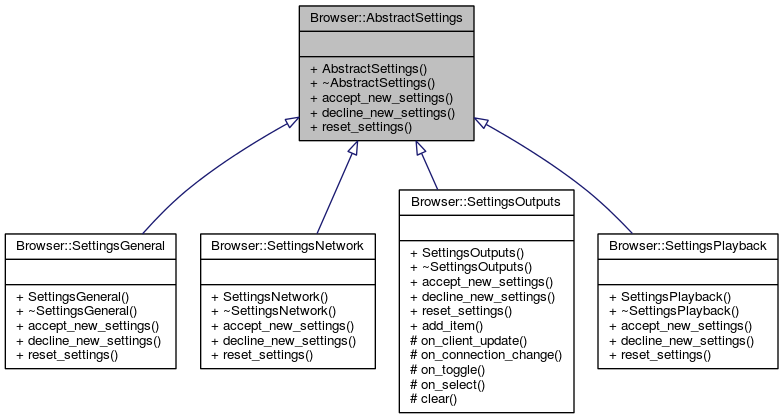
\includegraphics[scale=0.5]{AbstractSettings.png}
	\caption{Nutzer von AbstractSettings}
	\label{class_abstract_browser}
\end{figure}
Eine abstrakte Klasse die einen Reiter im Settingsbrowser repräsentiert. 
Sie soll die folgenden ,,pure virtual'' Methoden definieren:

\begin{verbatim}
    virtual void accept_new_settings(void)
\end{verbatim}
Weist Reiter an, alle Werte in die Config zu speichern
     
\begin{verbatim}
    virtual void decline_new_settings(void)
\end{verbatim}     
Weist Reiter an, die letzten validen Werte aus der Config zu laden

\begin{verbatim}
    virtual void reset_settings(void)
\end{verbatim}
Weist Reiter an, die Defaultwerte aus der einkompilierten Config zu laden.

\paragraph{Settings}
Die Settings Klasse repräsentiert den Settingsbrowser. Wie jeder andere Browser implementiert diese Klasse \emph{AbstractBrowser} und eine get\_container() Methode.
Sobald etwas in der Präsentation geändert wird, soll es nicht gleich in die Config übernommen werden.
Dies soll erst durch den Speicherbutton geschehen.
\begin{itemize}
\item Zurücksetzen - Setzt alle Einstellungen auf Fabrikstandards zurück
\item Rückgängig - Setzt Änderungen auf letzten Stand zurück
\item Speichern - Speichert aktuelle Änderungen
\end{itemize}

Die Klasse soll zudem eine Methode bieten um anzuzeigen, dass die ,,Settings'' geändert wurden z.B. durch Ausgrauen des Speicherbuttons:
\begin{verbatim}
    void settings_changed(void)
\end{verbatim}
Um in jeden Tab die Settings zurückzusetzen (auf letzten validen Wert oder Standardwert) speichert die Settingsklasse für jeden Reiter eine AbstractSettings Instanz in eine Liste. Sie kann so später darüber iterieren um die werte zu speichern, rückgängig zu machen oder zurück zu setzen. 

%<Zustandsdiagramm zum Settings akzeptieren, sprich buttons in/sens machen>

\paragraph{SettingsGeneral}
Die konkrete Klasse die den ,,General'' Tab implementiert.
Folgende Einstellungen sollen geändert werden können:
\begin{itemize}
\item ,,settings.libnotify.signal'' (checkbox)
\item ,,settings.libnotify.timeout'' (numberslider) (ausgegraut wenn 'signal' nicht aktiviert)
\item ,,settings.trayicon.tray'' (checkbox)
\item ,,settings.trayicon.totrayonclose'' (checkbox) (ausgegraut wenn 'tray' nicht aktiviert)
\end{itemize}

\paragraph{SettingsNetwork}
Die konkrete Klasse die den ,,Network'' Tab implementiert.
Folgende Einstellungen sollen geändert werden können:
\begin{itemize}
\item ,,settings.connection.port'' (numberslider)
\item ,settings.connection.host'' (stringentry)
\item ,,settings.connection.autoconnect'' (checkbox)
\item ,,settings.connection.timeout'' (numberslider)
\item ,,settings.connection.reconnectinterval'' (numberslider)
\end{itemize}
Zusätzlich soll ein Button zum Zeigen der Avahi-Serverliste angezeigt werden.

\paragraph{SettingsPlayback}
Die konkrete Klasse die den ,,Playback'' Tab implementiert.
Folgende Einstellungen sollen geändert werden können:
\begin{itemize}
\item Eine Einstellung zum ,,Crossfade'' (Überblendzeit). Diese wird vom Server gespeichert.
\item ,,settings.playback.stoponexit'' (checkbox)
\end{itemize}

\paragraph{SettingsOutputs}
Zeigt und verwaltet eine Liste von Outputs. Die Klasse benutzt die Funktion \textit{fill\_outputs()} von \emph{AbstractItemGenerator}
und muss daher von AbstractItemlist erben.

Wenn Änderungen übernommen werden, so wird über die Liste iteriert und für jeden Output entsprechend \emph{enable()} oder \emph{disable()} aufgerufen, 
falls der Output vorher aus-, respektive eingeschalten war.

\paragraph{OutputsModelColumns}
Die Spaltendefinition für die Outputliste.
Die Liste besteht aus dem Outputnamen (einem String), einer Anzeige ob der Aktiv ist (boolean),
und einen Pointer auf die AudioOutput Instanz um den entsprechenden Output en/disablen zu können.

\subsubsection{Statistics}
\paragraph{Statistics}
Eine Browserklasse die lediglich eine Reihe von Labels verwaltet und sie bei einem Clientupdate mit den aktuellen Server Statistiken.

Folgende ,,Statistics'' soll die Klasse darstellen:
\begin{itemize}
\item ,,Number of artists'' - Anzahl der Künstler in der Datenbank
\item ,,Number of albums'' - Anzahl der Alben in der Datenbank
\item ,,Number of songs'' - Anzahl der Songs in der Datenbank
\item ,,DB Playtime'' - Gibt die gesamte Spielzeit der Datenbank an
\item ,,Playtime'' - Seit wann abgespielt wird
\item ,,Uptime'' - Gibt an wie lange der Server läuft
\item ,,Most recent db update'' - Aktuellstes Datenbankupdate
\end{itemize}

Diese Informationen werden beim Start des Freya Clients und bei jedem Datenbankupdate abgerufen.
